
\documentclass[a4paper,12pt]{article}

\usepackage{graphicx} % Required for inserting images
\usepackage{amsmath,amssymb,amsfonts}
\usepackage{subcaption}
% -----------------------
% Package Imports
% -----------------------

% Set page margins
\usepackage[a4paper, top=1in, bottom=0.8in, left=1.1in, right=0.8in]{geometry}

% Use Times New Roman font
\usepackage{times}

% Add page numbering
\pagestyle{plain}

% Enable graphics inclusion
\usepackage{graphicx}
\usepackage{float}
% Enable code listings
\usepackage{listings}
\usepackage{xcolor} % For customizing code colors
\setlength{\parindent}{0pt}
\usepackage{titlesec} % Add this to your preamble
\titleformat{\section}
{\normalfont\large\bfseries}{\thesection}{1em}{}
% Set spacing for sections
\titlespacing*{\section}
{0pt}  % Left spacing
{0ex} % Space before (adjust this value)
{0.1cm}  % Space after (adjust this value)

\begin{document}
	\section{Experiment No. 5}
	
	\section{Experiment Title }
	Starting a DC Shunt Motor using 3 point starter
	\section{Objective}
	
	The objectives of this lab are as follows:
	\begin{itemize}
	\item To understand the construction and working of a 3-point starter in DC shunt motors.
	\item To observe the effect of back EMF on limiting the armature current as the motor gathers speed.
	\item To identify the limitations of a 3-point starter, especially in variable-speed motor applications.
	\end{itemize}
	
	\section{Theory}
	
	A three-point starter is an electrical device used to start and maintain the speed of a DC shunt motor. The circuit connects a resistance in series, which decreases the initial high current and protects the equipment from electrical failures. Back EMF (Electromotive Force) plays an essential role in operating the motor. As the motor's armature starts to rotate in the magnetic field, the back EMF is generated, opposing the supply voltage.\\
	
 
	Initially, the back EMF (\(E_b\)) is zero, but it gradually increases as the motor gathers speed. The general equation for the motor EMF is:
	
	\[
	E = E_b + I_aR_a
	\]
	
	Where:
	\begin{itemize}
		\item \(E\) is the Supply voltage,
		\item \(E_b\) is the Back EMF,
		\item \(I_a\) is the Armature current, and
		\item \(R_a\) is the Armature resistance.
	\end{itemize}
	
	Since \(E_b = 0\) at the start, the equation simplifies to:
	
	\[
	E = I_a R_a
	\]
	
	Thus, the armature current becomes:
	
	\[
	I_a = \frac{E}{R_a}
	\]
	
	As the armature resistance \(R_a\) is small, the initial current can be dangerously high, requiring the use of a device like the 3-point starter to limit the starting current to an acceptable value.
	
	
	
\begin{figure}[H]
	\centering

	\label{fig:construction-of-3-point-starter}
\end{figure}
	\begin{figure}[H]
		\centering
		\begin{subfigure}[t]{0.49\textwidth}
			\centering
			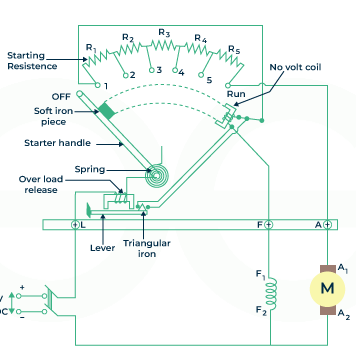
\includegraphics[width=1.2\linewidth]{Images/Construction-of-3-Point-Starter}
		\caption{Construction of 3 Point Starter}
		\end{subfigure}
		\hfill
		\begin{subfigure}[t]{0.48\textwidth}
			\centering
			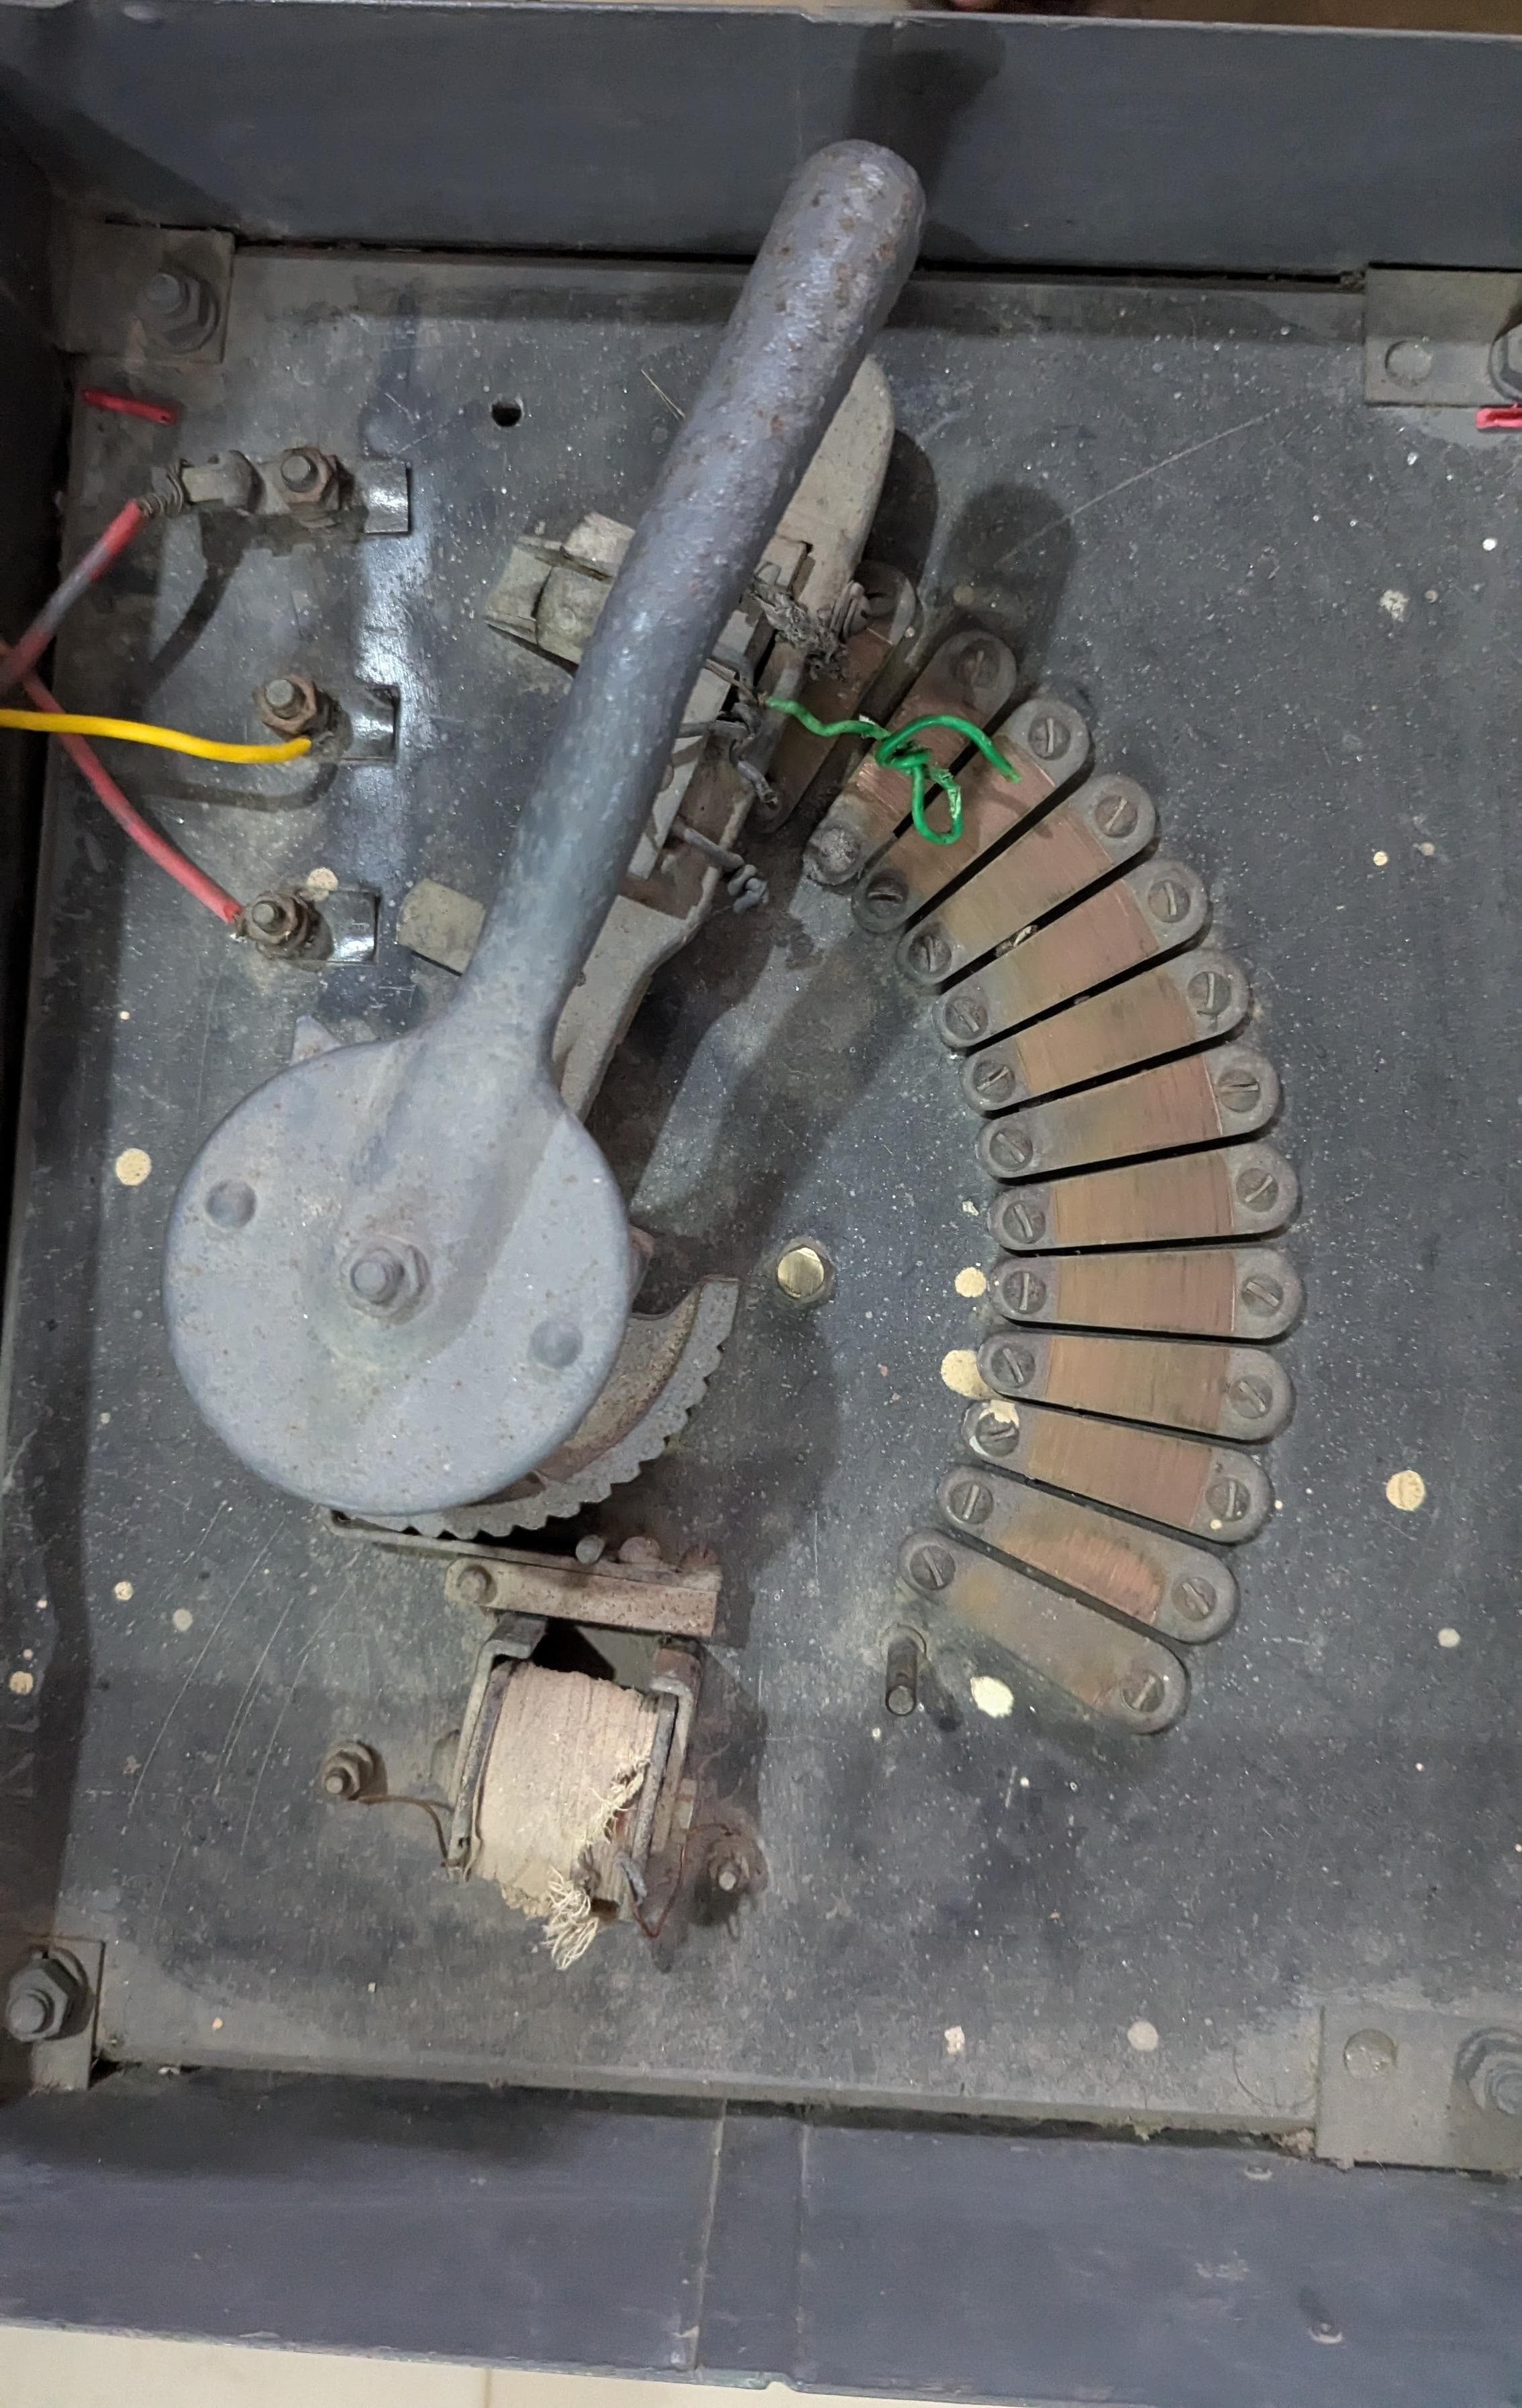
\includegraphics[width=0.7\linewidth]{Images/3ps}
			\caption{ 3-Point-Starter}
		\end{subfigure}
		
		\caption{Long Shunt and Short Shunt }
	\end{figure}
	
	\subsection{Construction of 3-Point Starter}
	
	The construction of a 3-point starter is a variable resistance integrated into several sections, denoted by contact points labeled OFF, 1, 2, 3, 4, 5, and RUN, called studs. The primary points in the circuit are:
	\begin{itemize}
		\item \(L\) – Line terminal (connected to the positive supply),
		\item \(A\) – Armature terminal (connected to the armature winding), and
		\item \(F\) – Field terminal (connected to the field winding).
	\end{itemize}
	
	This is why it is called a 3-point starter. The starter includes devices such as an overload release (OLR) and a no-volt coil (NVC) to protect the motor.
	
		\begin{figure}[H]
		\centering
		\begin{subfigure}[t]{0.49\textwidth}
			\centering
			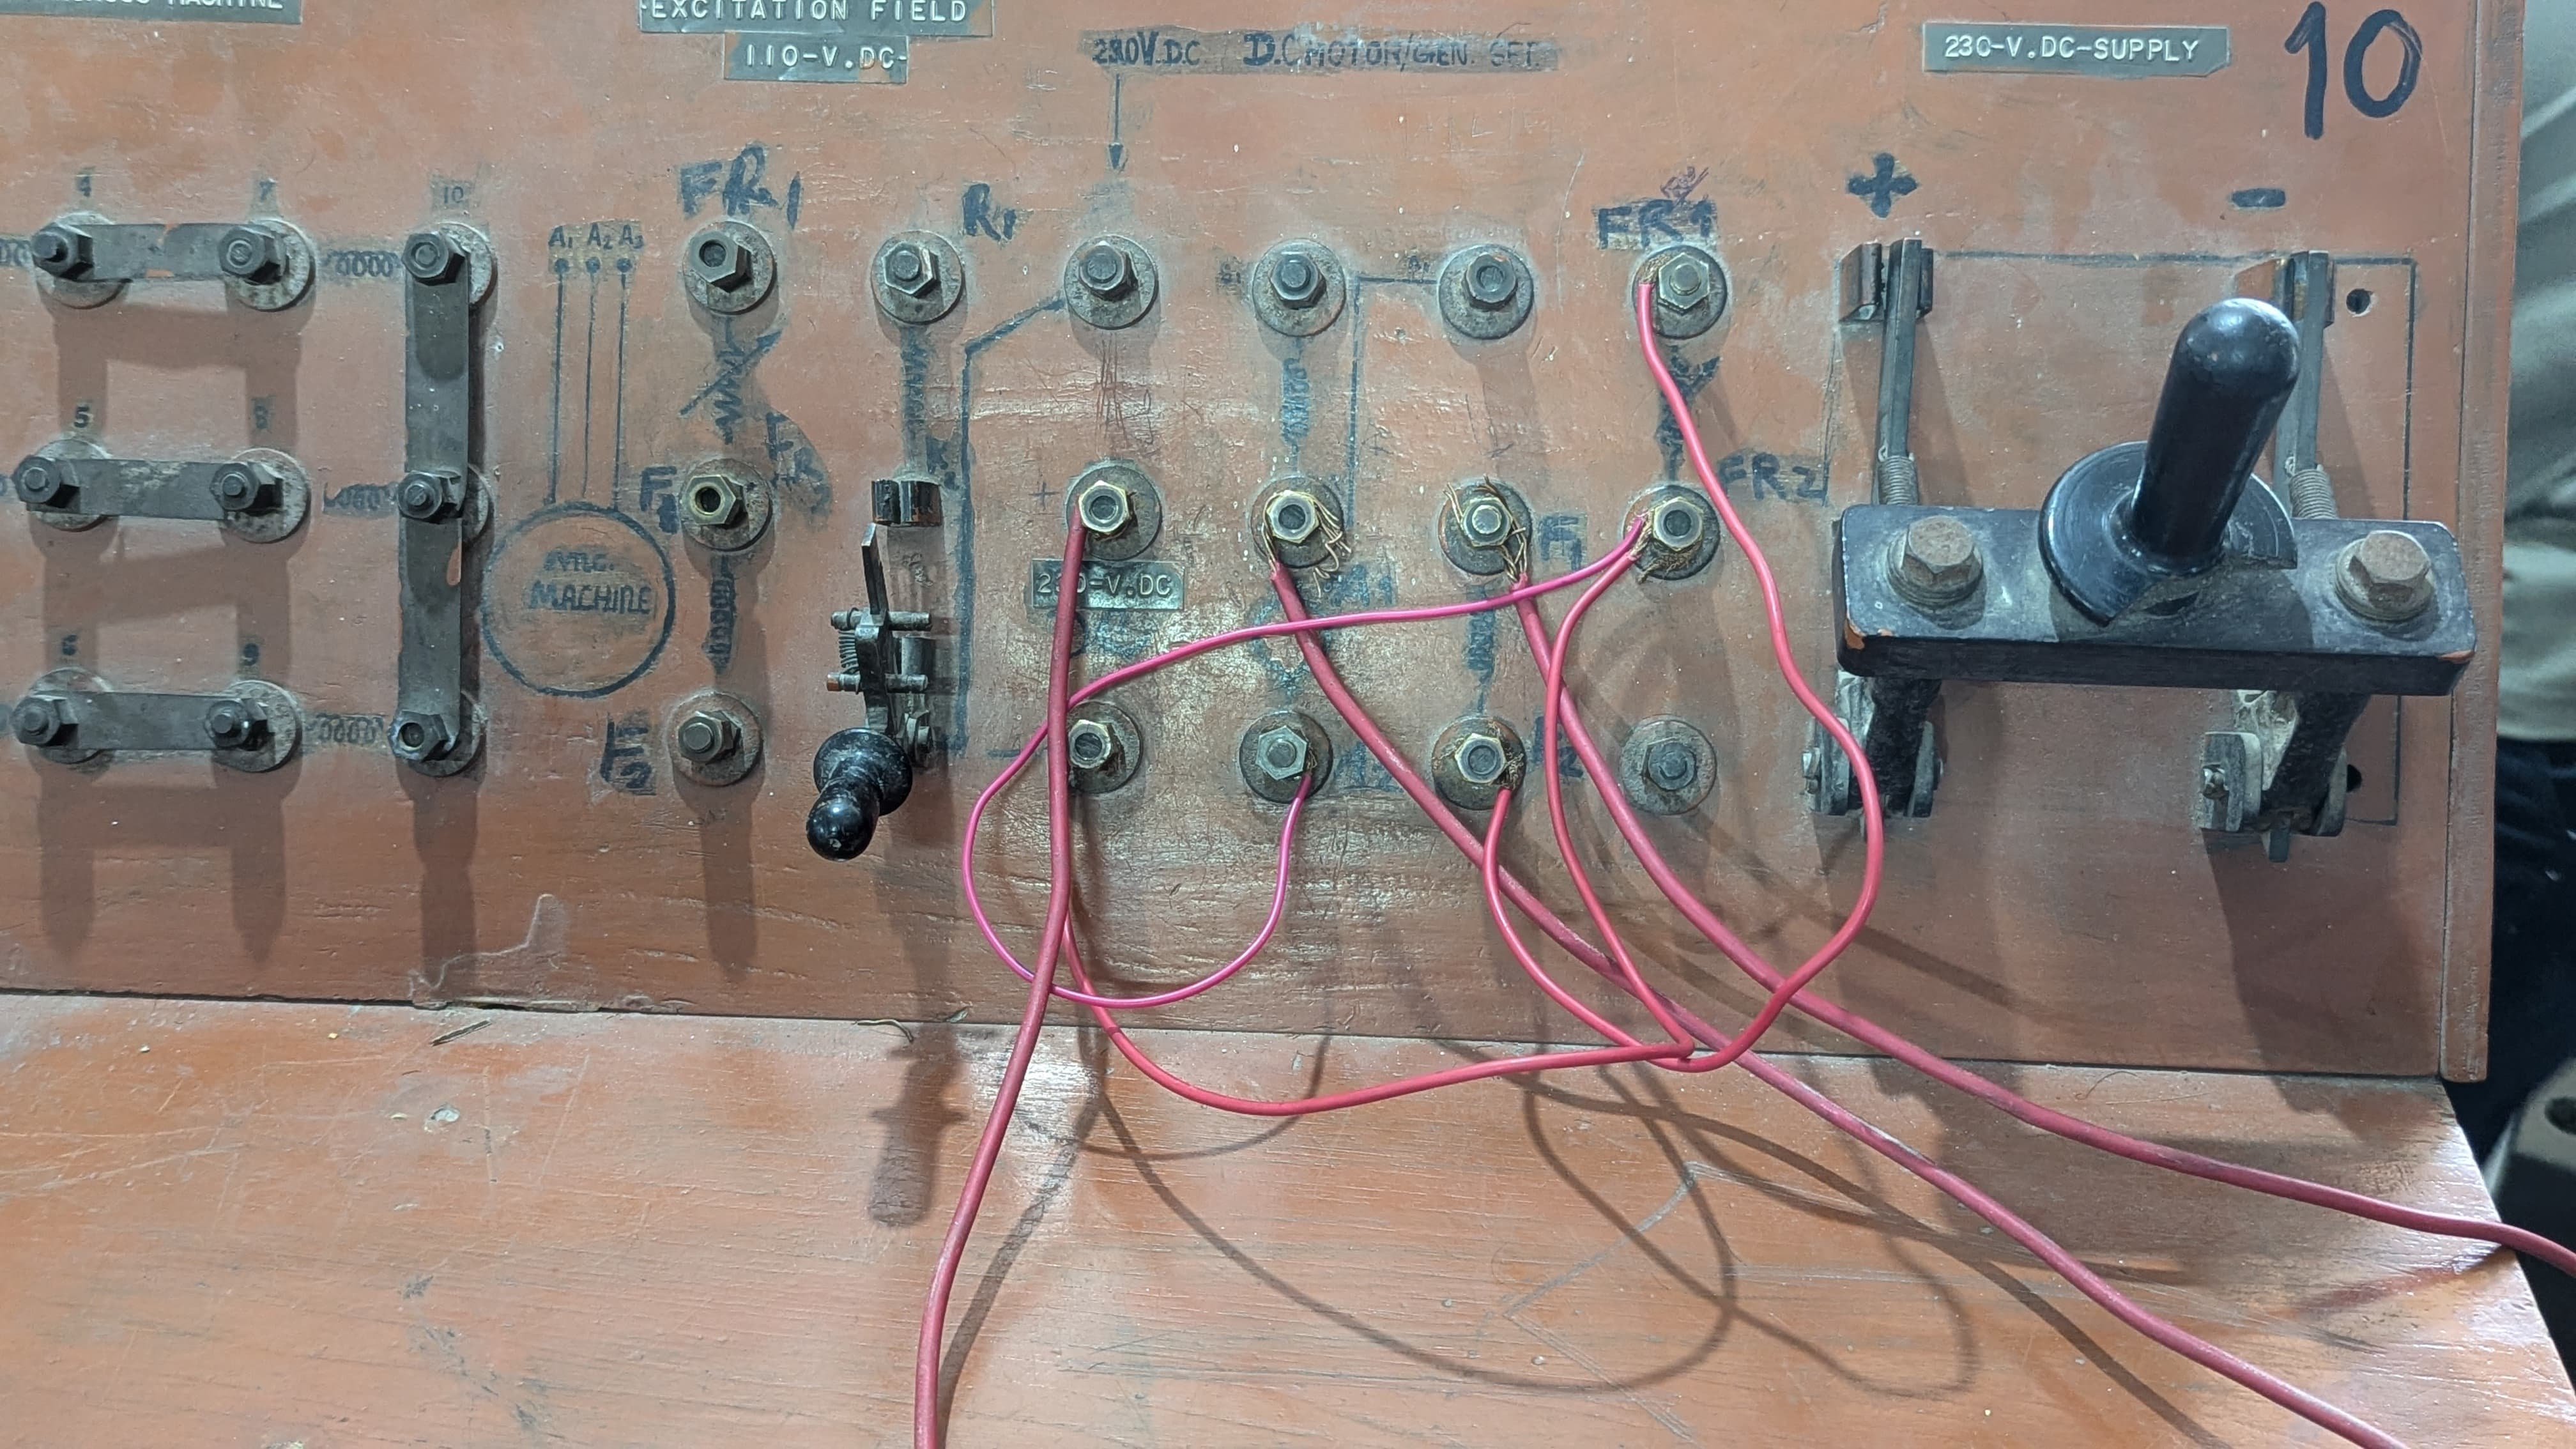
\includegraphics[width=1\linewidth]{Images/3pscrkt}
			\caption{Connection of DC Motor using 3 point starter}
		\end{subfigure}
		\hfill
		\begin{subfigure}[t]{0.48\textwidth}
			\centering
			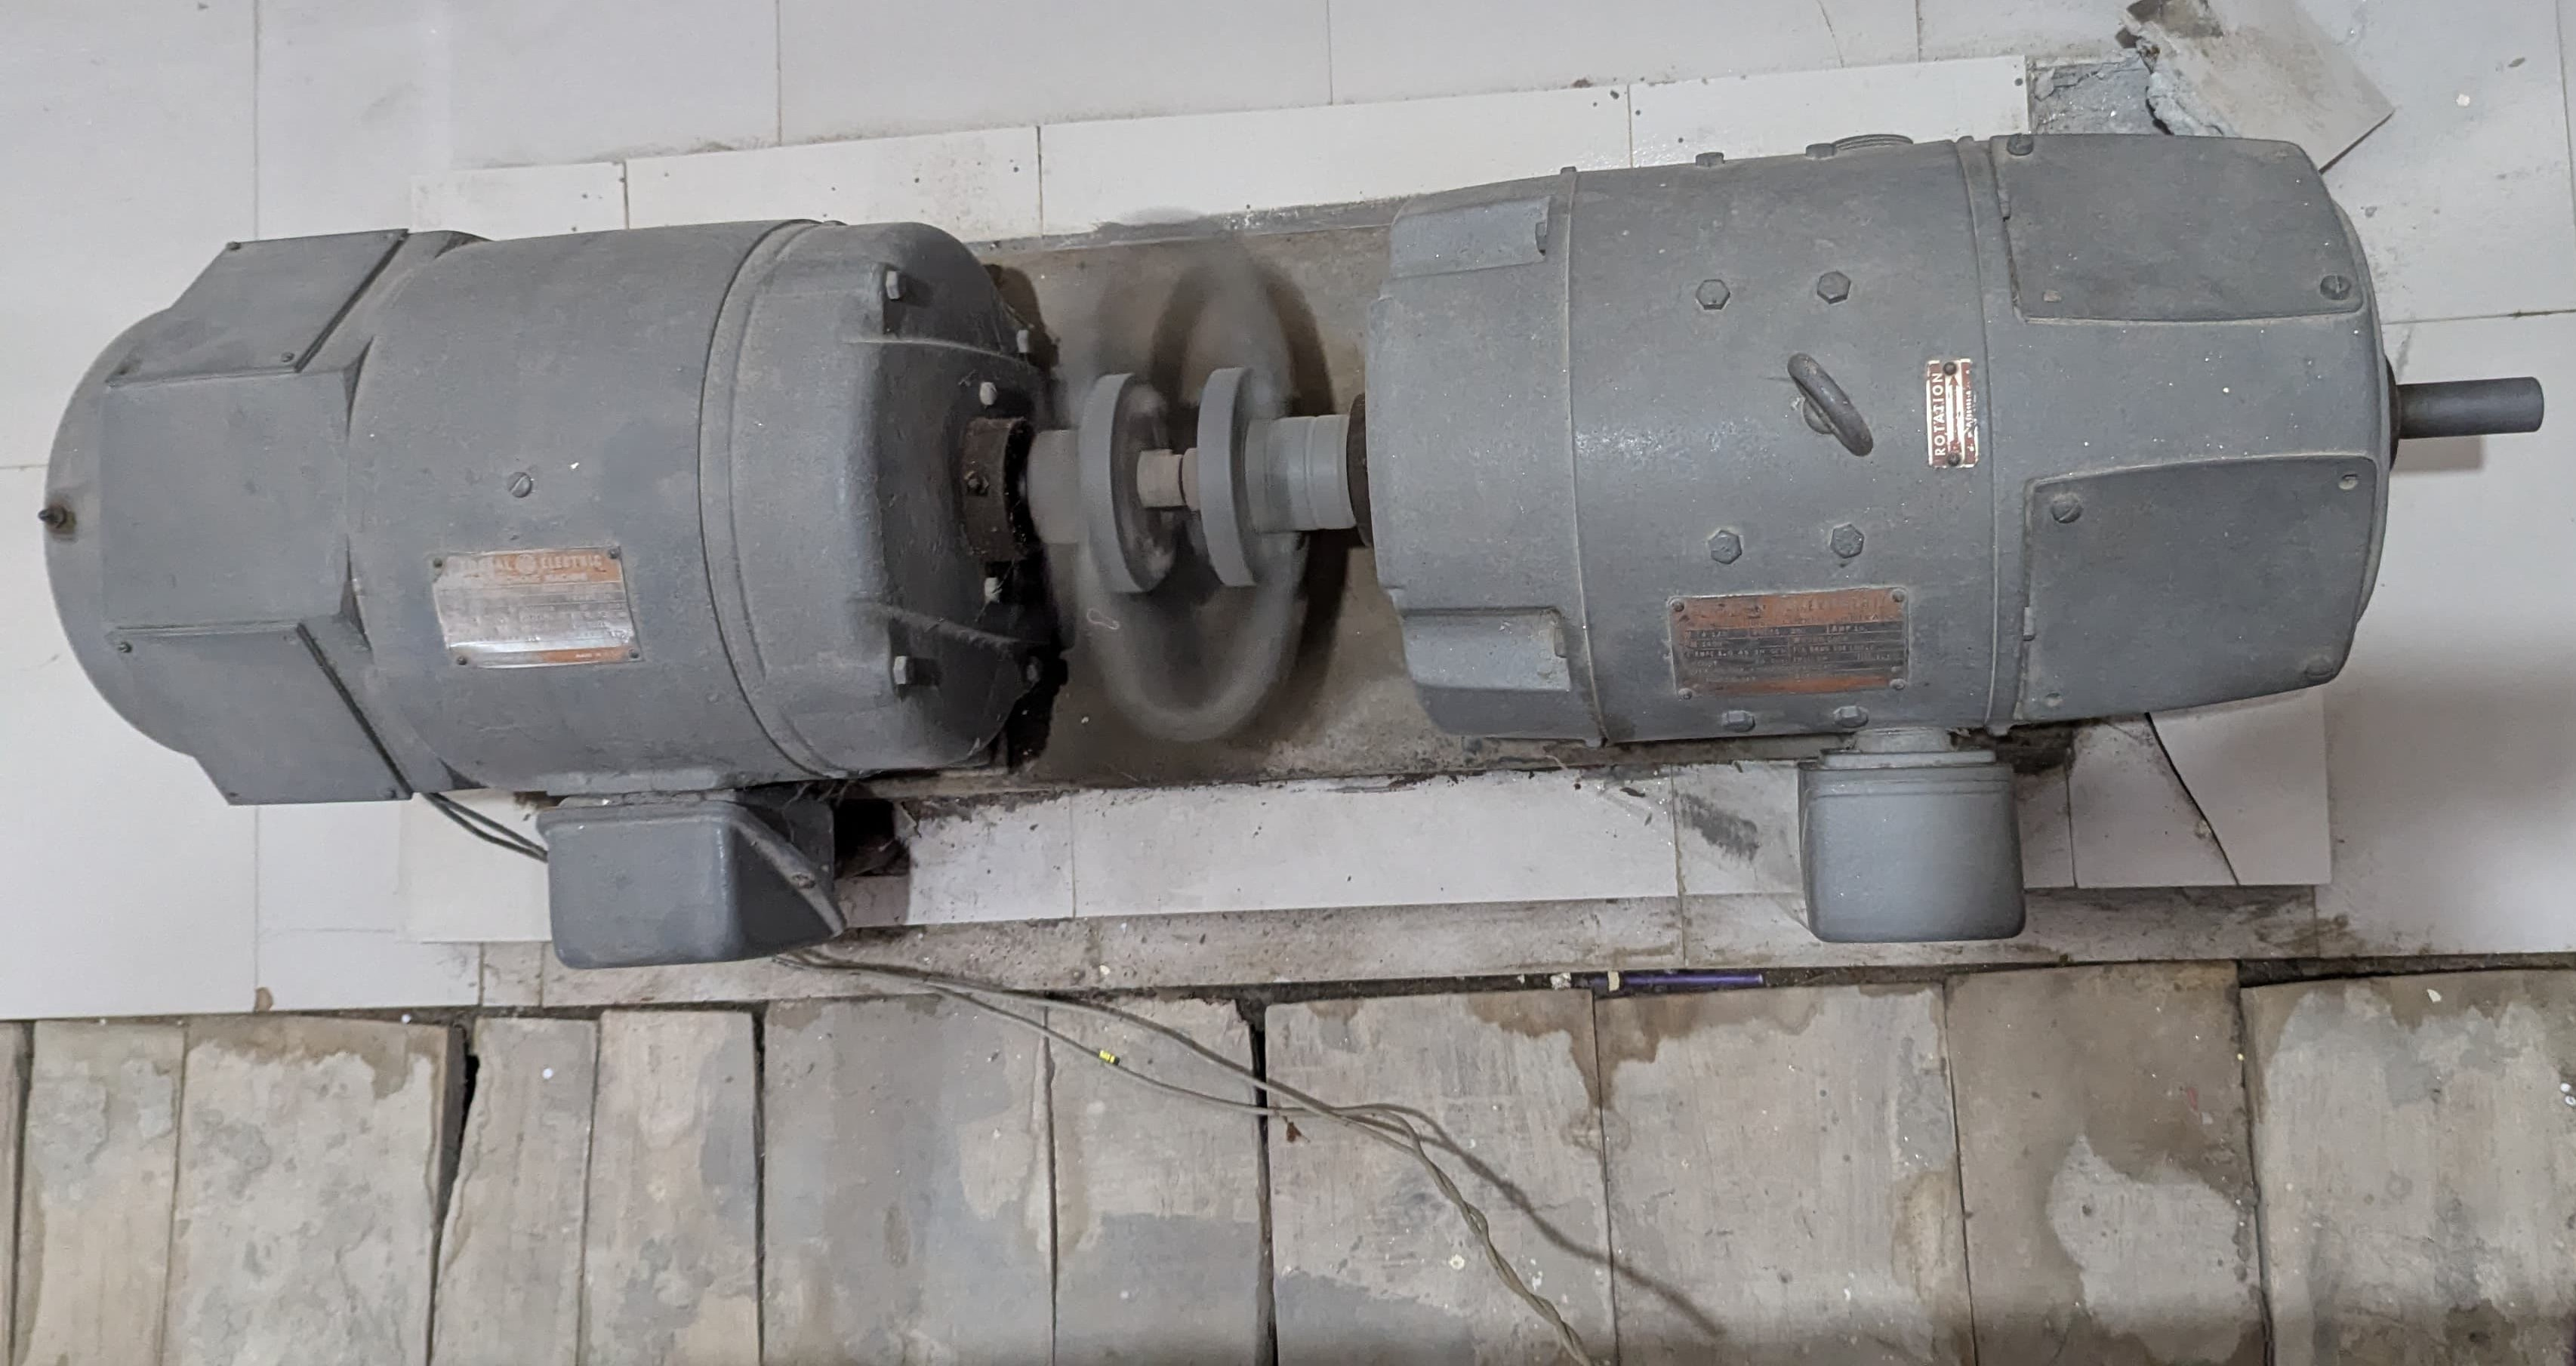
\includegraphics[width=1\linewidth]{Images/mtr}
			\caption{ DC Motor}
		\end{subfigure}
	\end{figure}
	\subsection{Working of 3-Point Starter}
	
	Initially, the handle is set to the OFF position. When power is supplied, the handle is gradually moved to engage the contacts of the studs (starting with stud 1). The field winding receives power through the parallel path, while the initial resistance is connected in series with the armature, limiting the high starting current. As the handle is moved toward the RUN position, resistance is gradually removed from the armature circuit.
	
\textbf{Back EMF and Motor Operation:}
	As the motor picks up speed, back EMF develops, countering the supply voltage, which reduces the armature current. The external resistance is no longer required for optimal operation, and the motor runs at its normal speed. 
	

\subsection{Functions of No-Volt Coil (NVC)}
At the point when the motor reaches at the normal speed and the arm is reached at the ON position, the entire starting resistance is cut off from the circuit. Now in running condition, assuming that the supply is interrupted or disconnected, the starting arm remains at the ON position. Additionally, the armature winding is connected directly across the primary supply when the supply is restored, so there is no back EMF in the circuit.\\
The NVC protects the motor in case of supply interruption. If the supply is cut off, the NVC coil de-energizes, allowing the spring to pull the starter handle back to the OFF position. This prevents a high inrush of current when the supply is restored.
	
	\subsection{Functions of Overload Release (OLR)}
	
	The OLR protects the motor from excessive current due to overload. When overload occurs, the high current flowing through the OLR coil pulls the armature upward, short-circuiting the NVC and pulling the handle to the OFF position, disconnecting the motor from the supply.
	
	\subsection{Advantages of 3-Point Starter}
	
	\begin{enumerate}
		\item Reduces high starting current.
		\item Provides motor speed control.
		\item Protects the motor from short circuits and overloads.
	\end{enumerate}
	
	\subsection{Disadvantages of 3-Point Starter}
	
	\begin{enumerate}
		\item Not suitable for variable-speed motors.
		\item Field current adjustments can disengage the NVC, causing the motor to disconnect from the supply.
		\item While increasing the high resistance from accomplish a high speed, the field current will always be extremely low.
		\item The holding electromagnet will not have the option to persevere through the power of the spring on the off chance that the field current is generally low.
	\end{enumerate}
	
	
	
	
	\section{Required Apparatus}
		\begin{enumerate}
		\item Three point Starter,
		\item DC Supply (230V),
		\item Connecting Wires,
		\item \textbf{Synchronous Machine} (Model 5SJ4254A2Y12,1500rpm, 1 PF,120/240 Volts 22/11 FL Amp, Field Amp MAX 2.1A ,Field Volts 125)  and  \textbf{Direct Current Generator} (250V,18 Amp,Comp Wound,1450 rpm) 
		
	\end{enumerate}

	\section{Circuit Diagram}

	\begin{figure}[H]
	\centering
	\begin{subfigure}[t]{0.9\textwidth}
		\centering
	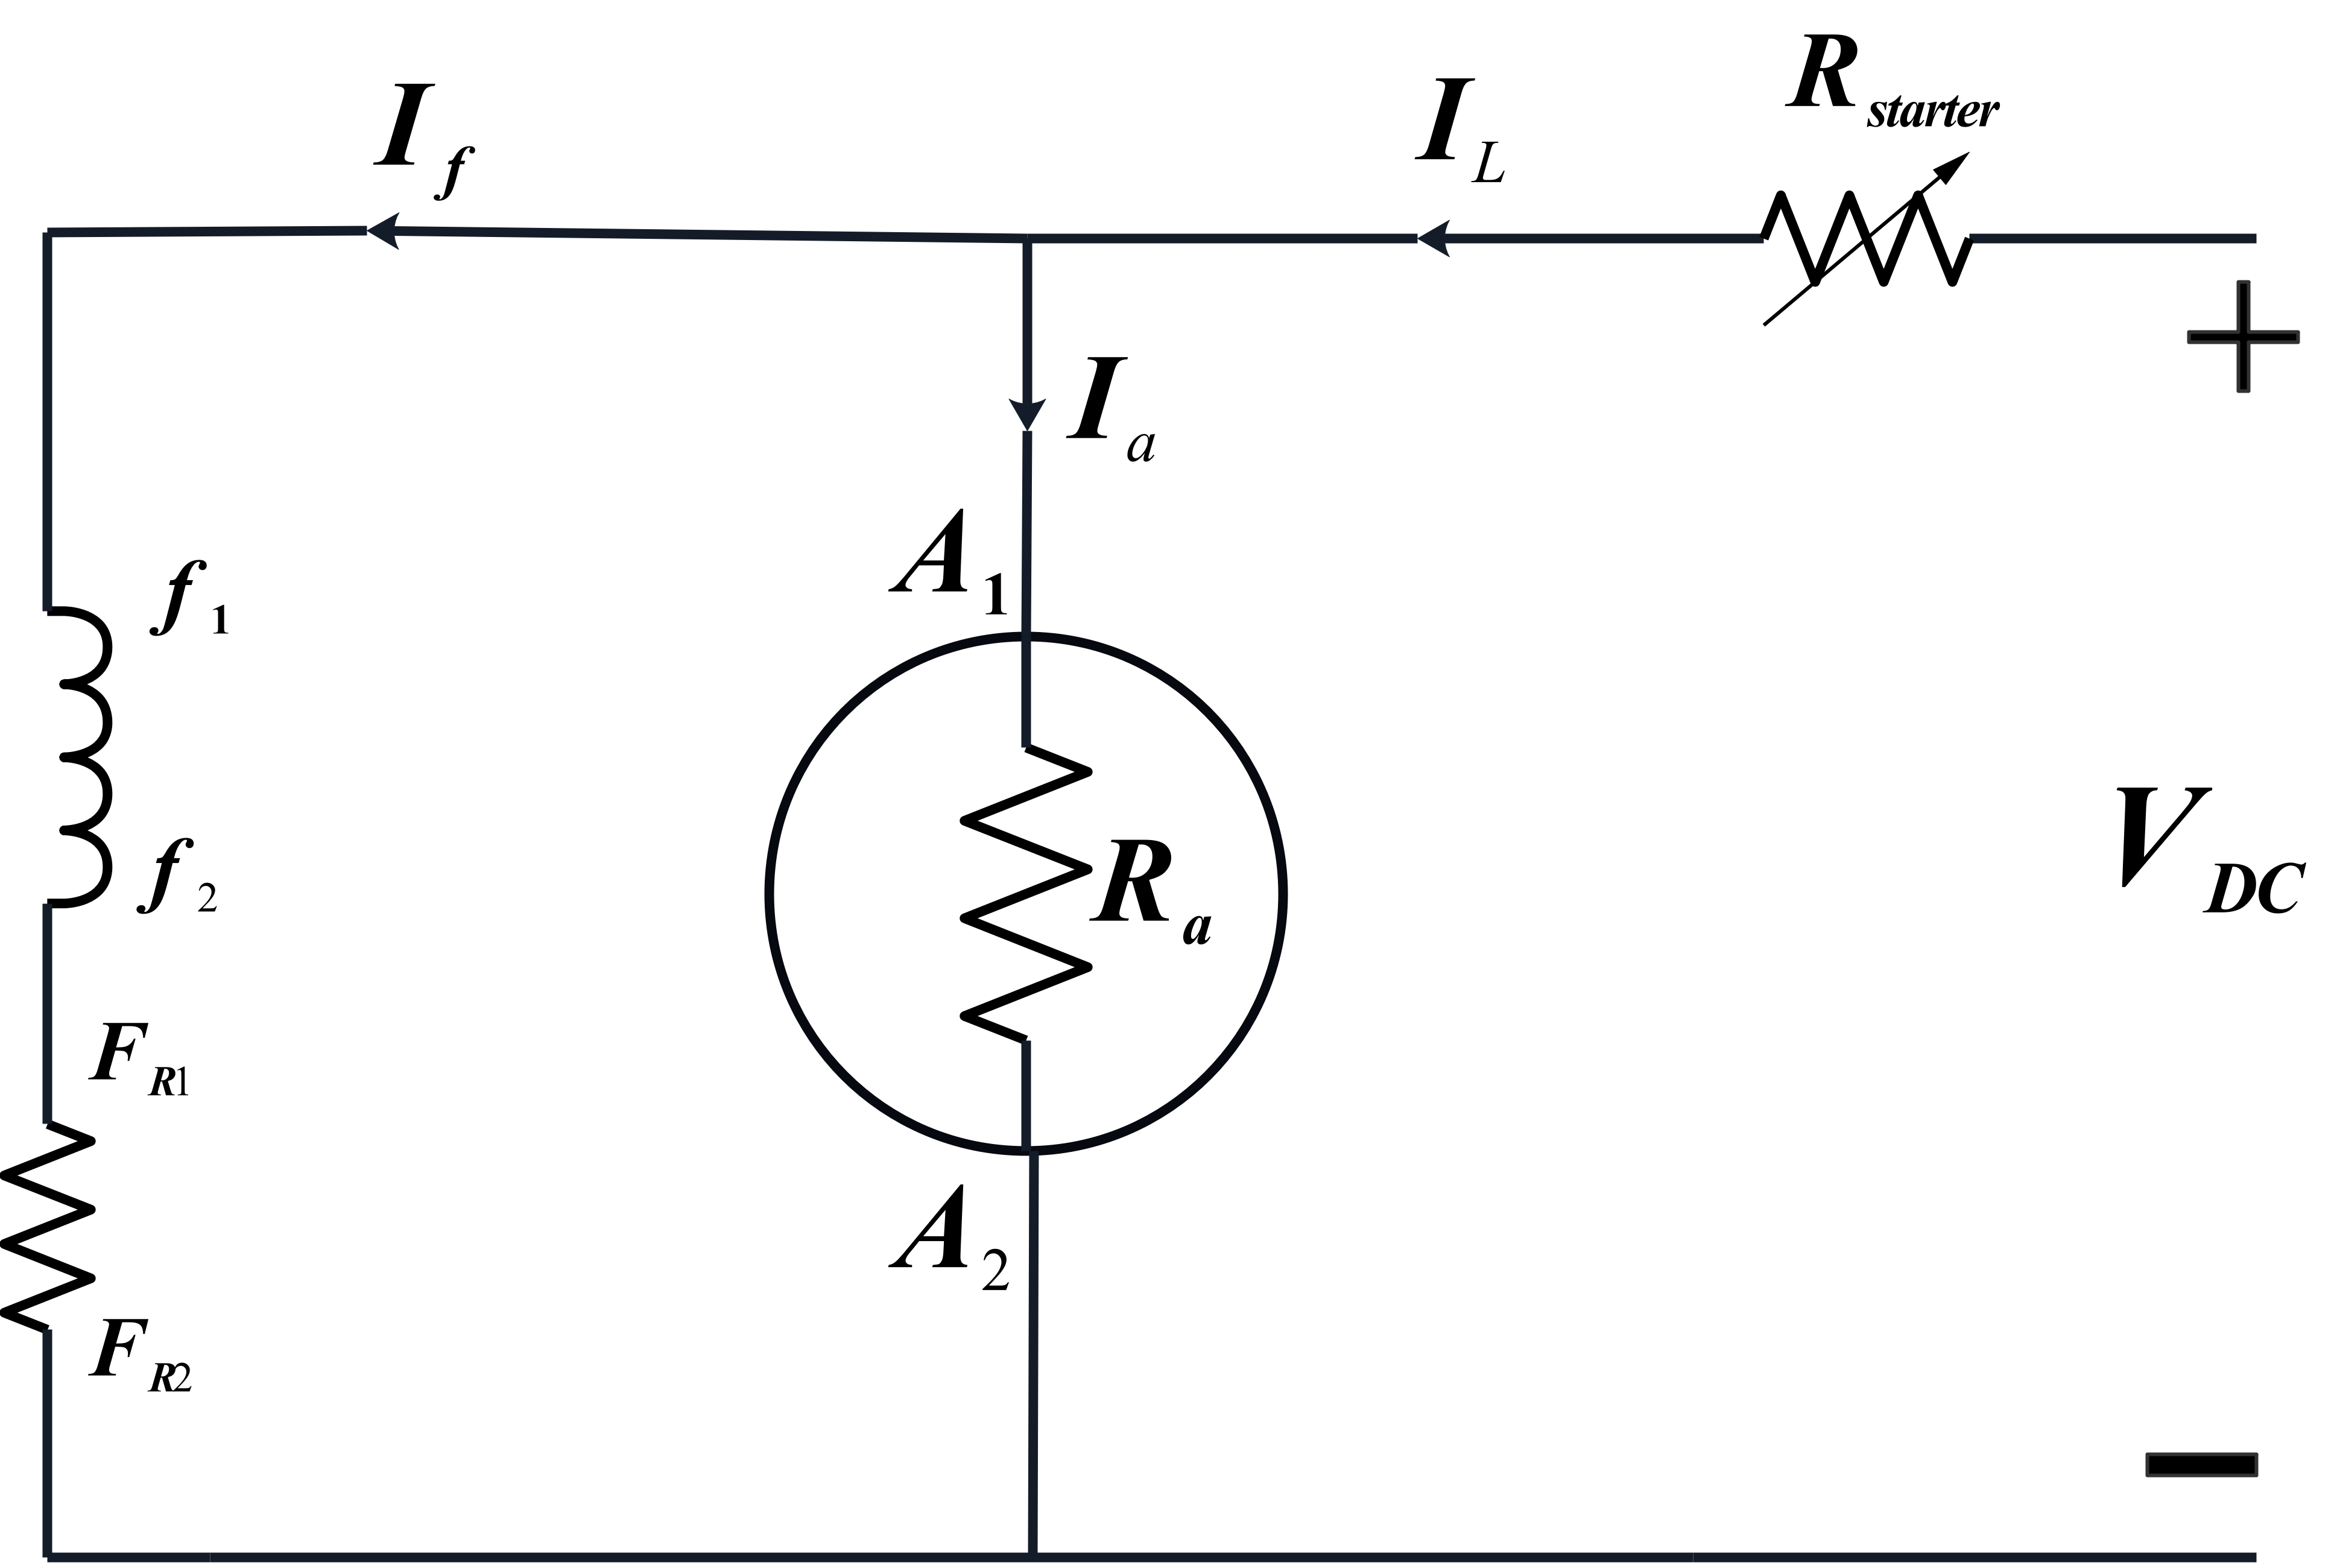
\includegraphics[width=.7\linewidth]{Images/Drawing06}
	\caption{Required Circuit Diagram}
	\vspace{0.1cm}
	\end{subfigure}

	\begin{subfigure}[t]{1\textwidth}
		\centering
		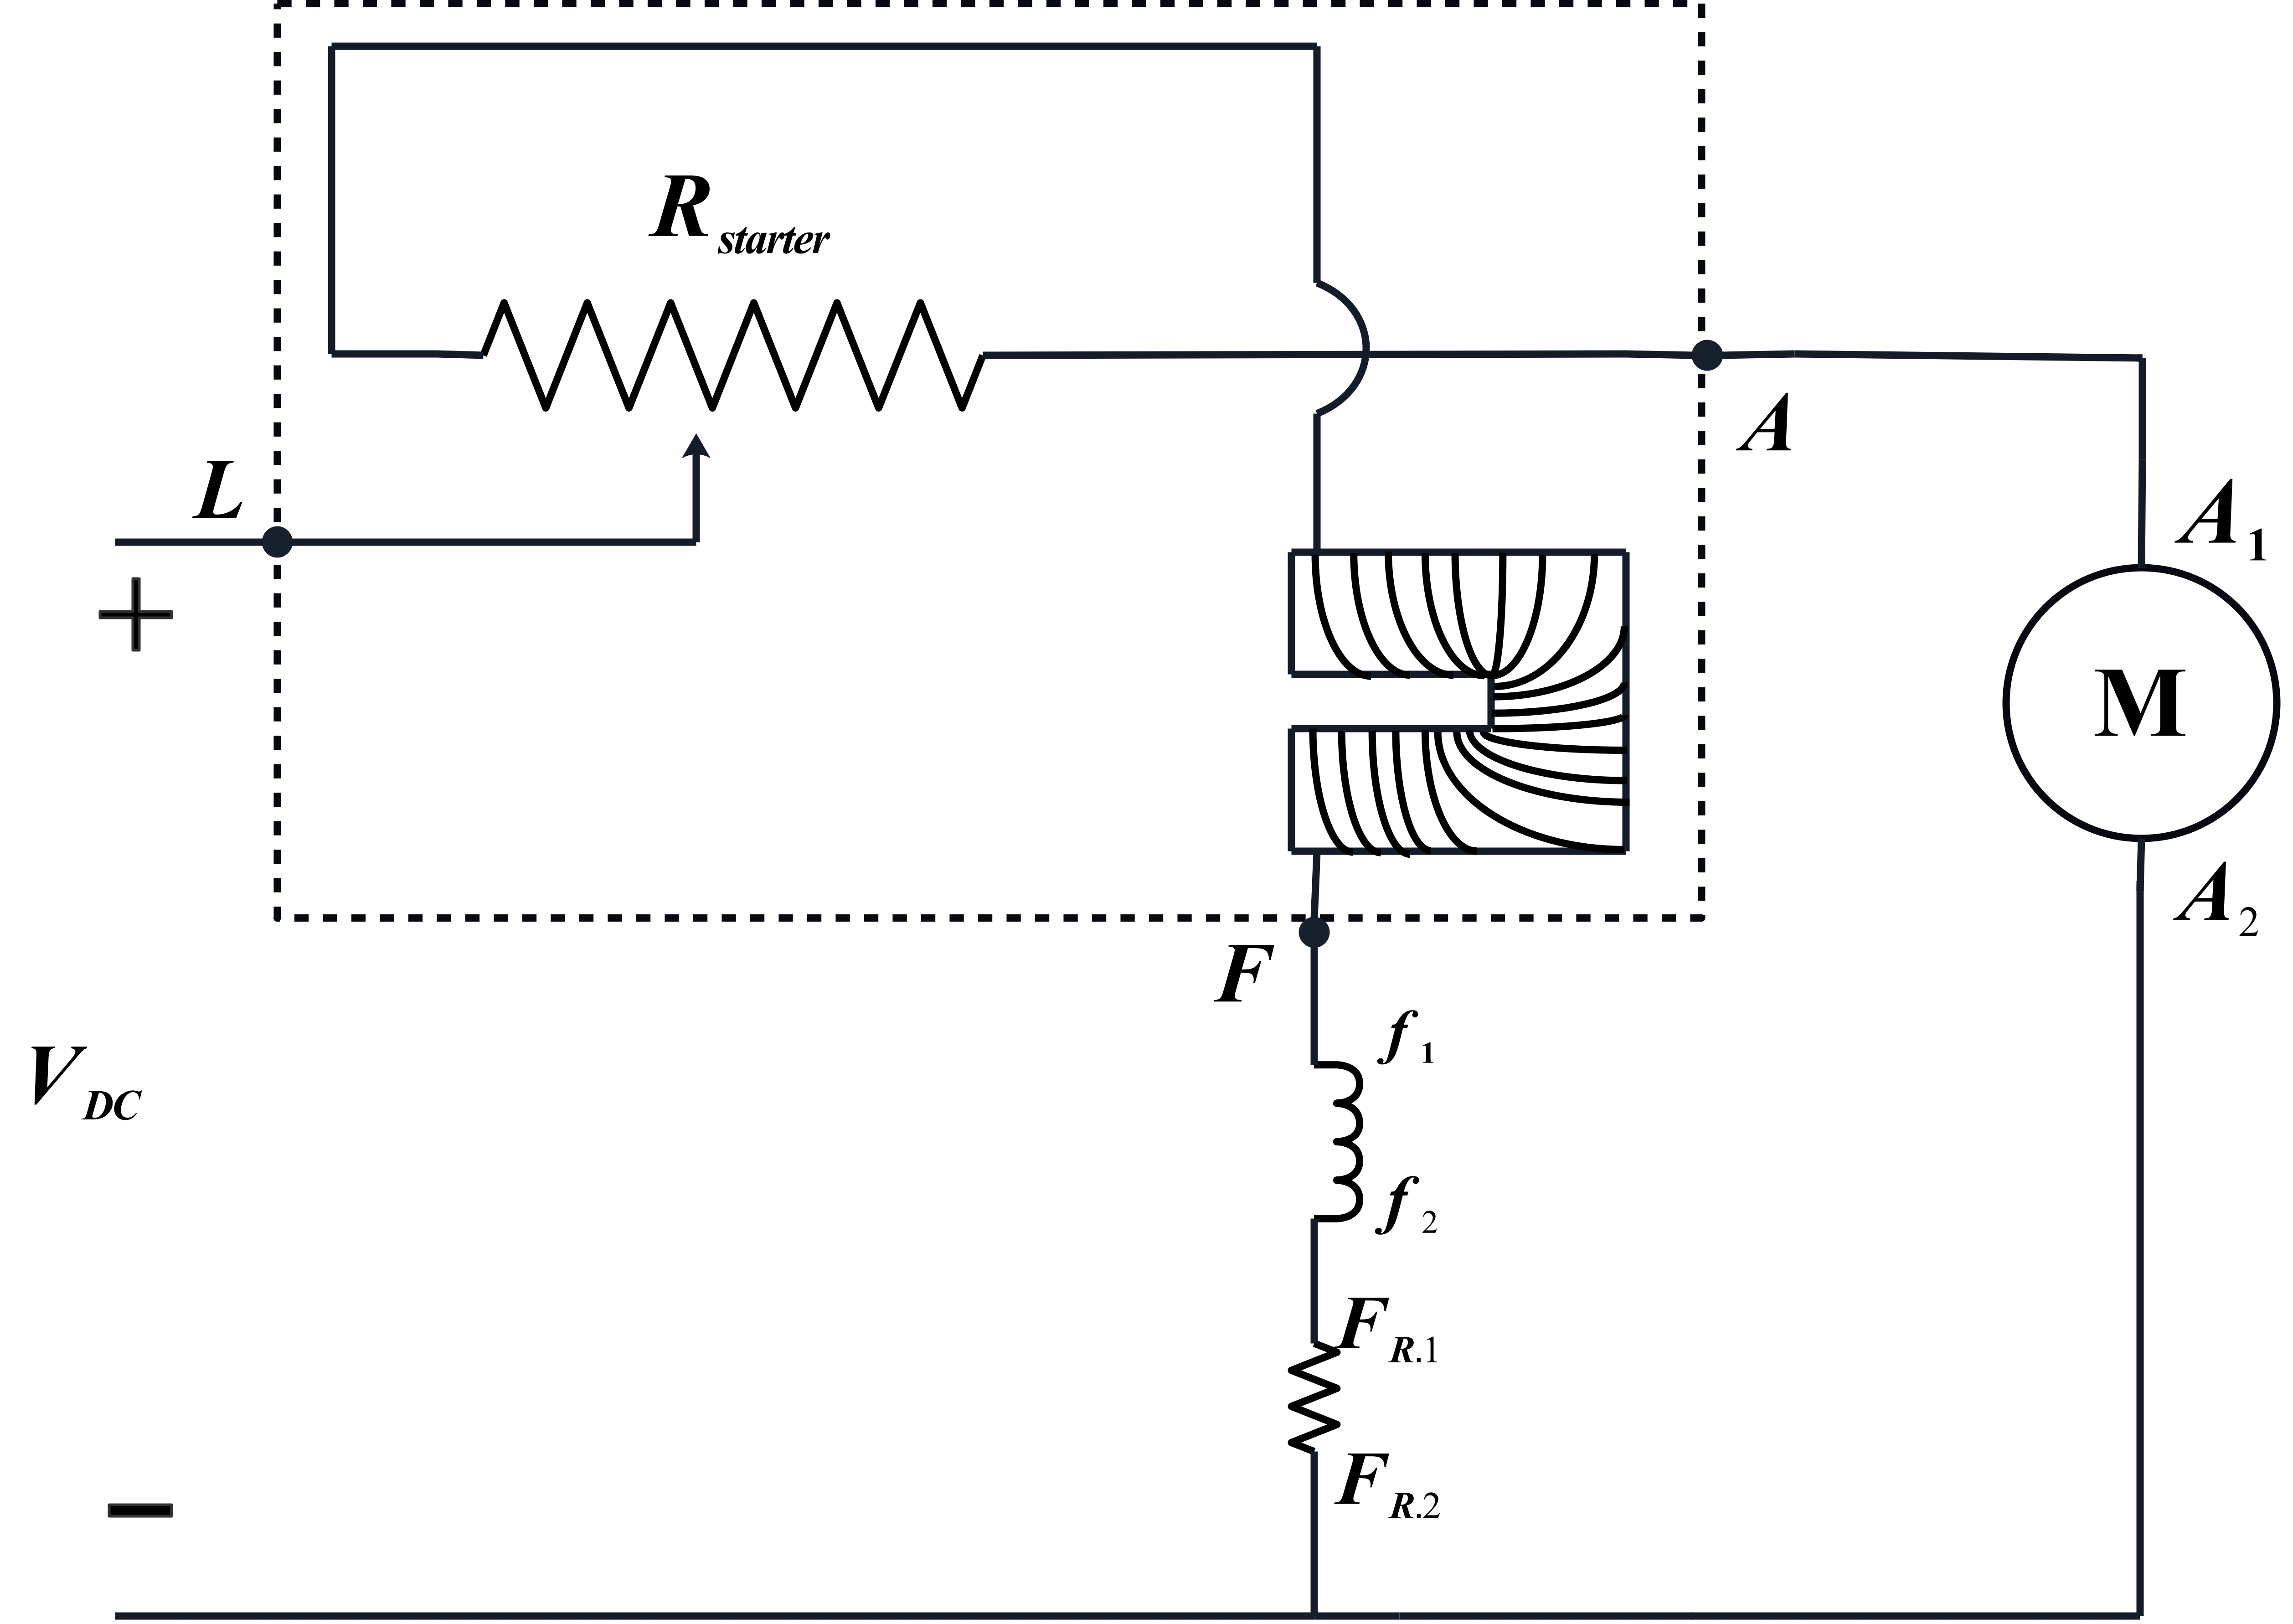
\includegraphics[width=0.9\linewidth]{Images/Drawing05}
	\caption{Connection of DC Shunt Motor using 3 point starter}
	\end{subfigure}
\end{figure}

\section{Discussion}
During the experiment, several key aspects of the operation of a 3-point starter for DC shunt motors were observed. It was noted that the 3-point starter played a critical role in limiting the high starting current by introducing series resistance. This protection was necessary because, at the moment of startup, no back EMF was present, which would have allowed the armature current to rise dangerously high due to the low armature resistance.

The behavior of back EMF was also closely monitored. As the motor began to rotate, the back EMF gradually increased, opposing the applied voltage and reducing the armature current. This relationship between back EMF and motor speed was crucial for ensuring the motor operated safely and efficiently, as confirmed by the equation:
\[
E = I_a \cdot R_a + E_b
\]
It was observed that the 3-point starter effectively managed this process by gradually reducing the series resistance as the motor gained speed.

The experiment further revealed the importance of protective mechanisms such as the No-Volt Coil (NVC) and Overload Release (OLR). These components automatically disconnected the motor from the power supply during abnormal conditions, such as supply failure or overload. This safety feature helped prevent damage to the motor's armature windings and ensured long-term operational stability.


In summary, the experiment successfully demonstrated the functioning and necessity of the 3-point starter in DC shunt motors, with particular emphasis on current regulation during startup and the role of protective devices in safeguarding the motor.

	
\end{document}